\section{RAG (Retrieval-Augmented Generation)} \label{sec:rag}

Il \emph{Retrieval-Augmented Generation} è il paradigma che Lewis et al. \cite{lewis2020retrieval} propongono per superare i due limiti discussi nella Sezione~\ref{sec:problema}: invece di affidarsi esclusivamente alla conoscenza codificata nei parametri del modello, il sistema recupera prima, da una base documentale esterna e aggiornabile, i frammenti (in inglese \emph{chunk}) di testo più pertinenti alla domanda ricevuta, e li fornisce al modello linguistico come contesto su cui basare la risposta. Il principio di fondo è separare nettamente \emph{cosa il sistema sa}, cioè l'insieme dei documenti indicizzati, che può essere aggiornato in qualunque momento senza bisogno di un nuovo addestramento, da \emph{come il sistema si esprime}, compito che resta demandato interamente al modello linguistico. Gao et al. \cite{gao2023ragsurvey}, nella loro rassegna sul tema, inquadrano questo principio come la risposta più diretta proprio ai limiti di conoscenza statica e di verificabilità discussi in precedenza: un'affermazione generata dal modello può essere ricondotta a un frammento di testo specifico, citabile e verificabile, invece che
derivare implicitamente e in modo opaco dai suoi parametri. La figura \ref{fig:rag-pipeline} mostra quella che è una pipeline generica di un sistema RAG.

\begin{figure}[H]
  \centering
  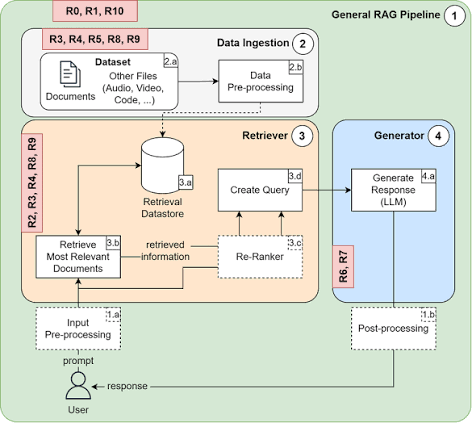
\includegraphics[width=0.6\textwidth]{assets/rag_pipeline.png}
  \caption{Schema generale di una pipeline RAG (1). Nella fase di \emph{data ingestion} (2), i documenti
  e gli altri file della collezione (2.a) vengono pre-elaborati (2.b) e indicizzati in un archivio per il
  recupero (3.a). Al momento della domanda, il prompt dell'utente viene eventualmente pre-elaborato (1.a) e
  passato al \emph{retriever} (3), che recupera i documenti più pertinenti (3.b), li riordina facoltativamente
  tramite un \emph{re-ranker} (3.c) e costruisce la richiesta da inviare al modello (3.d). Il
  \emph{generator} (4) produce la risposta tramite un LLM (4.a), che può essere post-elaborata (1.b) prima di
  essere restituita all'utente. I riquadri tratteggiati indicano componenti opzionali.}
  \label{fig:rag-pipeline}
\end{figure}

\subsection{Embedding e ricerca per similarità}\label{subsec:embedding}

Il primo problema che un sistema RAG deve risolvere è, dato un testo, come rappresentarlo in una forma che permetta
di confrontarne il significato con quello di una domanda. La soluzione standard è l'\emph{embedding}: una rete neurale
proietta ogni porzione di testo (un documento, o più spesso un suo frammento) in un vettore di numeri reali di
dimensione fissa, costruito in modo che frammenti dal significato simile vengano proiettati in punti vicini dello
spazio vettoriale. La vicinanza tra due vettori $\mathbf{u}$ e $\mathbf{v}$ si misura tipicamente con la
\emph{similarità coseno}, ovvero il coseno dell'angolo compreso tra i due vettori:
\begin{equation}
  \cos(\mathbf{u}, \mathbf{v}) = \frac{\mathbf{u} \cdot \mathbf{v}}{\lVert \mathbf{u} \rVert \, \lVert \mathbf{v} \rVert},
  \label{eq:coseno}
\end{equation}
che vale 1 per vettori con la stessa direzione e diminuisce man mano che le loro direzioni divergono.

Il punto di partenza per costruire modelli di embedding è in genere Bidirectional Encoder Representations
from Transformers (\emph{BERT}), proposto da Devlin et al.\ \cite{devlin2019bert}. A differenza dei LLM generativi descritti in precedenza, BERT utilizza solo la parte \emph{encoder} del Transformer: ogni token osserva
l'intera sequenza in entrambe le direzioni, e il modello produce per ciascun token un vettore che ne rappresenta il
significato nel contesto, senza generare testo. BERT viene pre-addestrato su grandi quantità di testo a ricostruire
parole mascherate casualmente all'interno delle frasi, e poi specializzato tramite \emph{fine-tuning} su compiti di
comprensione del linguaggio: la classificazione di un testo (per esempio l'analisi del sentiment), il riconoscimento
di entità nominate come persone e luoghi, l'individuazione della risposta a una domanda all'interno di un passaggio
dato, e la classificazione di coppie di frasi, per esempio per stabilire se due frasi sono parafrasi l'una dell'altra.

Nessuno di questi compiti, tuttavia, richiede di produrre un singolo vettore che rappresenti un'intera frase, e BERT
non è addestrato a farlo. Per confrontare due testi, BERT li riceve concatenati in un'unica sequenza e restituisce un
punteggio per la coppia, secondo un'architettura detta \emph{cross-encoder}. Reimers e Gurevych \cite{reimers2019sbert}
osservano che questo approccio è impraticabile per il recupero: ogni coppia richiede un passaggio completo attraverso
la rete, e trovare la coppia più simile in una collezione di 10.000 frasi richiede circa 50 milioni di passaggi, pari a
circa 65 ore di calcolo. D'altra parte, ricavare un vettore per ciascuna frase da BERT così com'è, per esempio facendo
la media dei vettori dei suoi token, produce embedding di bassa qualità.

La loro soluzione, Sentence-BERT (SBERT), affina BERT proprio per produrre embedding di frase confrontabili tramite la
similarità coseno. Durante l'addestramento, i due testi di ogni coppia non vengono concatenati, ma attraversano
separatamente la stessa rete, con gli stessi pesi; i due vettori risultanti vengono confrontati, e l'errore commesso
nel valutare la relazione tra i due testi (per esempio, se si tratta di parafrasi) viene usato per aggiornare i pesi.
Questa configurazione è detta \emph{siamese}, perché equivale a due copie gemelle della stessa rete. La condivisione dei
pesi garantisce che entrambi i testi vengano trasformati dalla stessa funzione, e quindi proiettati nello stesso
spazio, mentre l'addestramento fa sì che in questo spazio la similarità coseno rifletta la somiglianza di significato.
Una volta addestrata, la rete può calcolare l'embedding di ogni frammento una sola volta e indipendentemente dagli altri,
e il confronto con una domanda si riduce a una similarità coseno tra vettori già pronti: il tempo necessario a trovare
la coppia più simile tra 10.000 frasi scende così da circa 65 ore a circa 5 secondi.

Sentence-BERT è pensato per misurare la somiglianza tra frasi; nel recupero, invece, occorre confrontare una domanda
breve con passaggi di testo più lunghi che ne contengono la risposta. Karpukhin et al.\ \cite{karpukhin2020dpr}
applicano lo stesso principio a questo compito con il \emph{Dense Passage Retriever} (DPR), composto da due encoder
basati su BERT, uno per le domande e uno per i passaggi, addestrati su coppie domanda-passaggio in modo che l'embedding
di una domanda risulti vicino a quello del passaggio che contiene la risposta. Gli autori mostrano come DPR superi nettamente i metodi lessicali classici come BM25, che assegna un punteggio a ciascun documento in base alle parole che ha in
comune con la domanda, pesate secondo la loro frequenza nel documento e la loro rarità nella collezione.

Il vantaggio deriva dal fatto che un retriever basato su embedding confronta significati e non parole: una domanda come
``quando si paga la seconda rata?'' può essere associata a un passaggio che parla di ``scadenza del secondo versamento'',
pur avendo con esso quasi nessuna parola in comune. Per questo i retriever basati su embedding vengono detti
\emph{densi}, in contrapposizione alle rappresentazioni \emph{sparse} dei metodi lessicali come BM25, che descrivono un
testo con un vettore grande quanto l'intero vocabolario e composto quasi interamente da zeri. I metodi lessicali
restano comunque competitivi quando conta la corrispondenza esatta di un termine, come nel caso di codici o nomi propri.

Una domanda e un documento vengono quindi confrontati non piu sulla
base delle parole esatte che condividono, ma sulla distanza tra i rispettivi vettori nello spazio
degli embedding, calcolato in modo efficiente anche su milioni di candidati tramite strutture
dati specializzate (indici vettoriali) mantenute da un database vettoriale dedicato.

Un confronto esaustivo di un vettore query con ogni singolo vettore indicizzato (ricerca
esatta) diventa proibitivo già a poche centinaia di migliaia di frammenti, ben al di sotto della  scala di molti corpora documentali reali. I database vettoriali si affidano a una ricerca approssimata del vicino piu prossimo, che rinuncia alla garanzia di trovare sempre il risultato esatto in cambio di un tempo di
ricerca molto piu basso. Malkov e Yashunin \cite{malkov2018hnsw} propongono uno degli schemi più diffusi a
questo scopo, Hierarchical Navigable Small World (HNSW): un grafo multilivello in cui ogni
nodo rappresenta un vettore indicizzato, organizzato in strati via via piu densi, in cui la ricerca parte dallo strato piu rado (pochi nodi, collegamenti a lungo raggio) e scende progressivamente verso strati piu fitti, restringendo il raggio di ricerca a ogni passo; un meccanismo che ottiene un tempo di ricerca che cresce in modo logaritmico con il numero $N$ di vettori
indicizzati, $O(\log N)$, invece che linearmente, $O(N)$, come nella ricerca esatta.

\subsection{Ricerca ibrida e fusione dei risultati}

La ricerca per sola similarità vettoriale (\emph{dense retrieval}), tuttavia, ha un punto debole noto: tende a
performare peggio dei metodi lessicali classici (in particolare \emph{BM25} \cite{robertson2009bm25}) proprio sui termini rari o molto specifici: un codice di corso, una sigla normativa, un nome
proprio, che un embedding generico fatica a distinguere ma che un confronto esatto di parole individua senza
ambiguità. La letteratura piu recente raccomanda perciò l'adozione della \emph{ricerca ibrida} (\emph{hybrid search}): eseguire in parallelo una ricerca densa e una ricerca lessicale sparsa,
e fonderne i risultati in un'unica classifica. Una delle tecniche di fusione più diffuse a questo scopo,  è la \emph{Reciprocal Rank Fusion} (RRF), proposta da Cormack et al. \cite{cormack2009rrf}: per ogni documento si guarda non il punteggio ottenuto nelle due ricerche, ma solo la sua \emph{posizione} in ciascuna classifica e si sommano gli inversi di queste posizioni per ottenere un punteggio finale. Un documento che compare ai primi posti in entrambe le classifiche ottiene così un punteggio alto, uno che compare in alto in una sola delle due un punteggio intermedio. Il vantaggio pratico di questo meccanismo è che permette di fondere le due classifiche senza dover rendere confrontabili i punteggi originali delle due ricerche, cosa altrimenti problematica, perché il punteggio di una ricerca densa e quello di una ricerca lessicale sono calcolati in modo diverso e non sono direttamente comparabili tra loro.
\subsection{Reranking}

Il risultato della ricerca ibrida è però, tipicamente, solo una prima scrematura. Per restare efficienti su un
indice di grandi dimensioni, entrambe le sue componenti valutano ciascun frammento senza che un modello lo legga
mai insieme alla domanda. BM25 si limita a contare le parole in comune; nella componente densa, l'embedding di
ciascun frammento viene calcolato una volta per tutte, in fase di indicizzazione e quindi prima ancora di conoscere
la domanda, e al momento della ricerca viene soltanto confrontato con l'embedding della domanda tramite la
similarità coseno (Sottosezione~\ref{subsec:embedding}). Il vettore di un frammento deve perciò riassumerne l'intero
contenuto senza sapere quale aspetto interesserà a chi interroga il sistema: un frammento sulle tasse universitarie
è rappresentato sempre dallo stesso vettore, sia che la domanda riguardi la scadenza della seconda rata, sia che
riguardi l'importo previsto per una specifica fascia di reddito. Questa compressione comporta inevitabilmente una
perdita di dettaglio, e un frammento solo genericamente pertinente può finire in cima ai risultati davanti a quello
che contiene davvero la risposta. Un secondo stadio, il \emph{reranking}, corregge questo limite impiegando un
\emph{cross-encoder}: un modello che riceve domanda e documento candidato concatenati in un unico input e ne stima
direttamente la pertinenza reciproca, a un costo computazionale più alto ma applicato solo al pool già ristretto dei
migliori candidati della prima fase. Nogueira e Cho \cite{nogueira2019bert} sono tra i primi a mostrare, adattando
BERT a questo compito, che un cross-encoder di questo tipo migliora in modo sostanziale la qualità del ranking finale
rispetto alla sola similarità vettoriale.

Il cross-encoder rappresenta un estremo: domanda e documento vengono elaborati insieme, e ogni token dell'una
può essere messo in relazione con ogni token dell'altro in tutti gli strati della rete, al prezzo di dover
ripetere l'intero calcolo per ogni coppia. Esistono però soluzioni intermedie, che ottengono un confronto più dettagliato di
quello tra due singoli vettori senza sostenere il costo di un cross-encoder. Khattab e Zaharia \cite{khattab2020colbert} propongono
con ColBERT un'alternativa intermedia, la \emph{late interaction}: invece di comprimere ogni testo in un unico
vettore, ogni token di domanda e documento mantiene il proprio embedding, e la similarità complessiva si ottiene
aggregando le similarità massime tra i singoli token delle due sequenze --- un calcolo più ricco della sola
similarità tra due vettori aggregati, ma più leggero di un cross-encoder pieno, perché gli embedding dei documenti
possono comunque essere pre-calcolati e indicizzati in anticipo, mentre un cross-encoder richiede di rielaborare
congiuntamente domanda e documento a ogni confronto.
\subsection{Trasformazione della query}

Finora si è assunto implicitamente che la domanda usata per il recupero sia esattamente il testo digitato
dall'utente. Questo non è sempre il caso migliore: una domanda formulata in modo colloquiale o ellittico (che, ad esempio, fa
riferimento allo scambio precedente in una conversazione) può essere lessicalmente distante dal testo
del documento che contiene effettivamente la risposta, anche quando quel documento è topicamente pertinente. La
letteratura ha esplorato diverse strategie per colmare questa distanza riscrivendo la domanda prima di usarla per il
recupero, invece di cambiare il modo in cui i documenti vengono rappresentati. Gao et al. \cite{gao2022hyde}, con
HyDE (\emph{Hypothetical Document Embeddings}), propongono di chiedere a un LLM di generare un documento ipotetico
che risponderebbe alla domanda --- un testo che può contenere imprecisioni o essere parzialmente inventato --- e di
usare l'embedding di \emph{questo} documento, anziché quello della domanda originale, per la ricerca per similarità:
un documento ipotetico, per quanto impreciso nei dettagli, tende a essere lessicalmente e stilisticamente più vicino
ai documenti reali pertinenti di quanto non lo sia la domanda originale, spesso formulata in modo molto più
sintetico.

Un problema distinto, riguarda le domande che esprimono più di una richiesta
informativa: un singolo
passaggio di recupero sulla domanda combinata rischia di restituire chunk pertinenti a una sola delle due richieste,
perché il reranking valuta ogni candidato contro l'intera domanda invece che contro le sue parti. Ammann et al.
\cite{ammann2025decomposition} affrontano esplicitamente questo caso con la \emph{decomposizione della domanda}: un
LLM scompone la domanda originale in una o più sotto-domande autonome, il recupero viene eseguito separatamente per
ciascuna, e i risultati vengono fusi e riordinati con un cross-encoder standard --- un approccio che gli autori
mostrano migliorare il recupero su benchmark di question answering multi-hop (cioè un insieme standard di domande con risposte note usato per confrontare sistemi diversi) in cui la risposta richiede di combinare informazioni contenute in documenti diversi, senza richiedere alcun addestramento
aggiuntivo o indicizzazione specializzata.
\subsection{Chunking e fusione gerarchica}

Un ultimo problema, trasversale a tutti gli stadi precedenti, è quello del \emph{chunking}: un documento specie se lungo, come un regolamento o una dispensa, non può essere indicizzato come unico blocco, sia per limiti di
lunghezza degli input dei modelli di embedding sia perché un frammento troppo esteso diluisce il segnale specifico
cercato dalla domanda in mezzo a informazione non pertinente. La scelta della dimensione dei frammenti è però essa
stessa un compromesso: frammenti troppo corti rischiano di perdere il contesto necessario a renderli comprensibili
in isolamento, frammenti troppo lunghi tornano a soffrire del problema opposto.

La strategia più semplice consiste nel suddividere il testo in blocchi di dimensione fissa, eventualmente con una
sovrapposizione tra blocchi consecutivi per non spezzare un'informazione a cavallo del confine. Questo approccio tuttavia ignora la
struttura logica del documento: un paragrafo coerente può essere tagliato a metà solo perché il conteggio dei token ha raggiunto la soglia impostata. Un'alternativa più sensibile al contenuto è il \emph{chunking strutturale}, che rispetta i confini naturali del documento (sezioni, paragrafi, righe di una tabella) invece di tagliare a una lunghezza fissa, cedendo una parte dell'uniformità dei frammenti risultanti in cambio di un testo internamente più coerente. Nessuna delle due strategie, da sola, risolve però il problema opposto: un frammento strutturalmente coerente ma troppo corto (un singolo titolo di sezione, una riga isolata di una tabella) resta comunque privo del contesto che lo renderebbe comprensibile se recuperato in isolamento.

Una soluzione a questo problema è la \emph{fusione gerarchica} dei frammenti. In fase di
indicizzazione ogni documento viene diviso in frammenti piccoli, che sono quelli effettivamente
indicizzati e confrontati con la domanda, ma si conserva anche il legame di ciascun frammento con
la sezione del documento a cui appartiene. Al momento del recupero, se tra i frammenti selezionati
ne compaiono abbastanza appartenenti alla stessa sezione, questi vengono sostituiti dalla sezione
intera: il recupero conserva così la precisione dei frammenti piccoli, mentre il modello riceve un
contesto ampio e coerente.

\subsection{Posizione del contesto nel prompt}

Un'ultima scelta, a valle di tutte quelle discusse finora, riguarda come assemblare nel prompt i frammenti
recuperati, ordinati per pertinenza: semplicemente concatenarli nell'ordine restituito dal reranking non è
necessariamente innocuo. Liu et al. \cite{liu2023lostmiddle} mostrano che un LLM non utilizza un contesto lungo in
modo uniforme: l'accuratezza nel reperire un'informazione specifica è più alta quando questa si trova all'inizio o
alla fine del contesto fornito, e cala sensibilmente quando si trova nel mezzo un andamento a U che gli autori
osservano persistere anche in modelli progettati esplicitamente per finestre di contesto lunghe, e che ricorda gli
effetti di primacy e recency studiati nella memoria umana(vedere la figura: \ref{fig:u-curve}).
\begin{figure}[H]
  \centering
  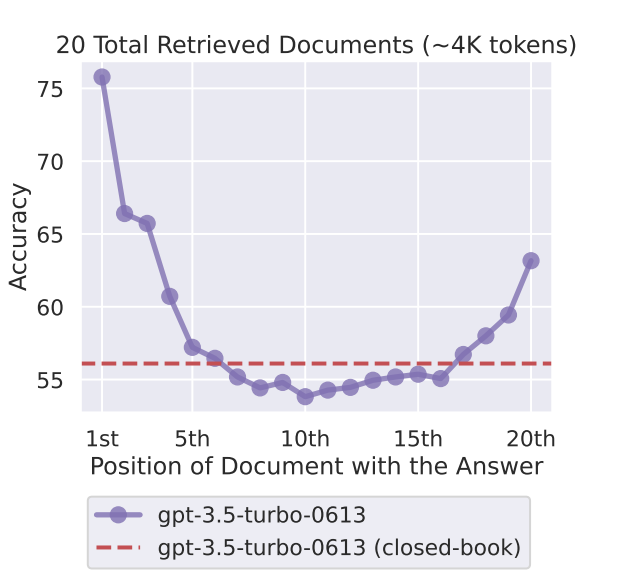
\includegraphics[width=0.5\textwidth]{assets/U-curve-diagram.png}
  \caption{La modifica della posizione delle informazioni rilevanti (in questo caso, la posizione del passaggio che risponde a una domanda in input) all'interno del contesto di input del modello linguistico produce una curva delle prestazioni a forma di U: i modelli sono più abili nell'utilizzare le informazioni rilevanti che compaiono all'inizio o alla fine del proprio contesto di input, e le prestazioni diminuiscono in modo significativo quando i modelli devono accedere e utilizzare informazioni situate nella parte centrale del proprio contesto di input. Fonte: Liu et al. \cite{liu2023lostmiddle} }
  \label{fig:u-curve}
\end{figure}

Per un sistema che costruisce il proprio contesto
unendo più frammenti recuperati, come quello di questo lavoro, questo risultato implica che l'ordine con cui i
frammenti vengono presentati al modello non è un dettaglio ininfluente quanto potrebbe sembrare a prima vista, specie
quando il numero di frammenti recuperati si avvicina al
limite superiore per cui l'effetto è stato osservato in letteratura.